\documentclass[conference]{IEEEtran}

\usepackage{graphicx} % For including images
\usepackage{amsmath} % For mathematical symbols and equations
\usepackage{hyperref} % For hyperlinks
\usepackage{caption}
\usepackage{amsfonts} % For math fonts and symbols
\usepackage{booktabs} % For better tables
\usepackage{listings} % For code listings
\usepackage{multirow} % For multi-row cells in tables

\begin{document}
	
	\title{Data Management \\ Project of a Data Warehouse System for Analyzing Meteorite Landings by NASA}
	
	\author{
		\IEEEauthorblockN{Giuseppe Valente - Natalia Maria Mucha}
		\IEEEauthorblockA{
			Engineering in Computer Science \\
			Sapienza University of Rome \\
		}
	}
	\maketitle
	
	\begin{abstract}
			This project focuses on developing a data warehouse system to integrate and analyze meteorite landing data from NASA. The objective is to demonstrate how to design and implement a data warehouse on a relational database using ETL processes, a dimensional fact model (DFM) schema, and Postgres SQL for deployment. 
	\end{abstract}
	
	\section{Introduction}
	
	This project aims to develop a data warehouse system specifically designed to integrate and analyze data on meteorite landings using NASA's Meteorite Landings dataset. The project’s objective is to demonstrate how to design and implement a data warehouse on a relational database platform using Postgres SQL. The process involves the application of Extract, Transform, Load (ETL) techniques to systematically collect, clean, and organize the data. Additionally, the project employs a Dimensional Fact Model (DFM) schema to structure the data in a way that supports in-depth analysis. \\ The result is a powerful tool for advancing the study of meteorites and their impacts on Earth.
	
	\section{Data warehouse}
	A data warehouse (DWH), is a system used for reporting and make data analysis. Is a central repository of integrated data from one or more sources (dataset or data source). They store current and historical data in one single place that are used for creating reports. This is beneficial for companies as it enables them to interrogate and draw insights from their data and make decisions.

	\section{System Architecture}
	The DWH architecture in general is composed by the following components:
	\begin{itemize}
		\item \textbf{Datasets:} are collections of structured data organized to support reporting, analysis, and decision-making. These datasets are derived from various sources and are typically organized in a way that optimizes them for querying and analysis. 
		\item \textbf{ETL:} stands for Extract, Transform, Load, which is a process used in data warehousing to move data from source systems to a data warehouse.
		\item \textbf{Primary DWH:} refers to the central, most important repository where an organization consolidates, stores, and manages its key business data for analysis and reporting. It is designed to support decision-making processes by providing a comprehensive view of data from various sources.
		\item \textbf{Data mart:} is a specialized subset of a DWH, designed to focus on a specific business area, department, or function. It is essentially a smaller, more focused version of a DWH that serves the needs of particular users or business units. 
		\item \textbf{Reconcilied data (three layer architecture only):} refers to data that has been verified, adjusted, and aligned to ensure consistency, accuracy, and completeness across various sources or systems. The process of reconciling data involves comparing and aligning data from different sources to resolve discrepancies and ensure that the data is accurate and reliable.
	\end{itemize}
	
	The components are organized in a two or three layers architecture: 	
	\subsection{Two-Layer Architecture (2LA)}
	The 2LA is an architecture composed by two mainly elements, the sources and the DWH. In this architecture the data marts are considerated as the "presentation layer" of the architecture. This architecture is very useful in organization from mid to large size. \\
	\subsection{Three-Layer Architecture (3LA)}
	In this architecture there is an additional layer, the reconcilied data layer, that it creates a common reference data model for a whole enterprise. At the same time, it sharply separates the problems of source data extraction and integration from those of DWH population. However the reconciled data leads to more replication of operational source data and the	design process is complicated. \\
			
	\subsection{Meteorite Landings - Architecture}
	\begin{figure}[htpb]
		\centering
		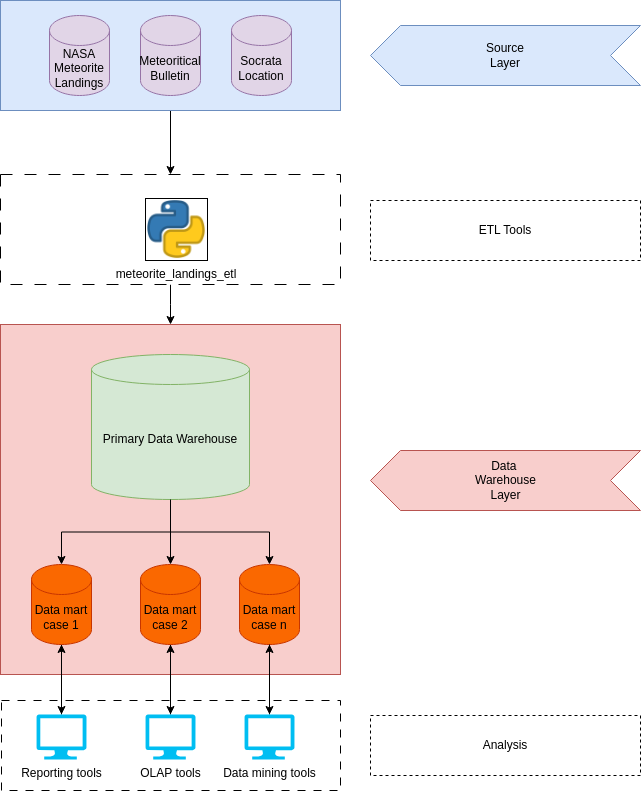
\includegraphics[width=\columnwidth]{images/system_architecture.png}
		\caption{Meteorite Landings System Architecture}
		\label{fig:Meteorite Landings System Architecture}
	\end{figure}
	We consider that for our purpose is better to use the 2LA, because we have not many data sources and then we can achieve the same result in this most simple way, because we can manage the enteire DWH system without using the Reconcilied Data.  In our architecture we identified the following components:
	\begin{itemize}
		\item \textbf{Datasets: (Meteorite Landings, Meteoritical Bulletin, Socrata Location)}
		\item \textbf{ETL: (extract.py, transform.py, load.py)}
		\item \textbf{Primary DWH: PostgreSQL}
		\item \textbf{Data marts: out of scope}  
	\end{itemize}
	
	\section{Source Layer}
	
	\subsection{Meteorite Landings Dataset}
	This comprehensive data set from The Meteoritical Society contains information on all of the known meteorite landings. The Fusion Table is collected by Javier de la Torre and we've also provided an XLS file that consists of 34,513 meteorites. \\
	\href{https://data.nasa.gov/Space-Science/Meteorite-Landings/gh4g-9sfh/about_data}{NASA's Open Data Portal}
	
	\subsection{Meteoritical Bulletin Database}
	This database has been constructed and is maintained by the Nomenclature Committee of the Meteoritical Society. The primary function of this database is to provide authoritative information about meteorite names. The correct spelling, complete with punctuation and diacritical marks, of all known meteorites recognized by the Meteoritical Society may be found in this compilation. Official abbreviations for many meteorites are documented here as well. The database also contains status information for meteorites with provisional names, and listings for specimens of doubtful origin and pseudometeorites. \\
	\href{https://www.lpi.usra.edu/meteor/}{Lunar and Planetary Institute}
	
	\subsection{Socrata Location}
	Dataset used to revert the coordinate point from latitude,longitude to human readable format.
	\href{https://dev.socrata.com/docs/datatypes/location.html#}{Tyler Technologies - Socdata}
				
	\section{ETL tools}
	The tools are developed in python, each of them has a specific goal and we would dockeraize our python scripts to allowing an horizontal scale-up in case of the data to elaborate grows or we need more computation in the trasforming or loading. We think this could be a good techincal choise in the application lifetime. This is the reason why we will use the dockers to run our scripts. For the same reason we would make a phisical separation of each software/script, each of them should resolve only one task.   
	\subsection{Extract}
	Data extraction scripts are written in Python, using libraries like `pandas` to read and process data files.
	
	\subsection{Transform}
	The transformation process includes converting geo-coordinates to human-readable formats and normalizing data formats across all datasets.
	
	\subsection{Load}
	The transformed data is loaded into the relational database using SQLAlchemy in Python, ensuring that all datasets are correctly integrated for analysis.
	
	\section{Data warehouse Layer}
	
	\subsection{Dimensions Fact Model (DFM)}
	
	\subsection{Relational Database realization}

	\section{Conclusion}
	
	\section{Reference}
	
	
	
	
	
\end{document}
